\documentclass[a4paper,11pt]{book}

% TEMPLATE
% ----------------------------------------------------------------------
\usepackage[utf8]{inputenc}
\usepackage{geometry}
\geometry{
	a4paper,
	left=20mm,
	top=30mm,
	bottom=30mm,
}
\usepackage[hidelinks]{hyperref}
\usepackage{titlesec}
\usepackage{etoolbox}
\usepackage{chngcntr}
\usepackage{graphicx}
\usepackage{lipsum}
\usepackage{xcolor}
\usepackage{amsmath,amssymb,amsfonts}
\usepackage{fancyhdr}
\usepackage{booktabs}

\counterwithout{figure}{chapter}
\renewcommand\thesection{\arabic{section}}
\patchcmd{\thebibliography}{\chapter*}{\section*}{}{}
\renewcommand{\bibname}{References}
\bibliographystyle{plainnat}
\pagestyle{empty}
\titleformat{\chapter}[frame]{\normalfont}{}{10pt}{\LARGE\bfseries\filcenter}
\pagestyle{fancy}
\fancyhf{}
\pagestyle{fancy}
% \fancyhead[LE,RO]{}
% \fancyhead[RE,LO]{Modelling for Engineering \& Human Behaviour 2024}
% \fancyfoot[C]{\thepage}

\renewcommand{\theequation}{\arabic{equation}}
\renewcommand{\thefigure}{\arabic{figure}}
\renewcommand{\thetable}{\arabic{table}}
% ----------------------------------------------------------------------


% ==============================
% Imports from my paper
% ==============================
\usepackage{hyperref}
\usepackage{graphicx}
\usepackage{subcaption}
\usepackage{amssymb}
\usepackage{amsmath}
\usepackage{multirow}
\usepackage{relsize}
\usepackage[utf8]{inputenc}
\usepackage[capitalise]{cleveref}
\usepackage{algorithm}
\usepackage[noend]{algpseudocode}
\usepackage[section]{placeins}
\usepackage{booktabs}
\usepackage{url}

% For the TODOs
\usepackage{xcolor}
\usepackage{xargs}
\usepackage[colorinlistoftodos,textsize=footnotesize]{todonotes}
\newcommand{\todoin}{\todo[inline]}
% from here: https://tex.stackexchange.com/questions/9796/how-to-add-todo-notes
\newcommandx{\unsure}[2][1=]{\todo[linecolor=red,backgroundcolor=red!25,bordercolor=red,#1]{#2}}
\newcommandx{\change}[2][1=]{\todo[linecolor=blue,backgroundcolor=blue!25,bordercolor=blue,#1]{#2}}
\newcommandx{\info}[2][1=]{\todo[linecolor=OliveGreen,backgroundcolor=OliveGreen!25,bordercolor=OliveGreen,#1]{#2}}

%Boldtype for greek symbols
\newcommand{\teng}[1]{\ensuremath{\boldsymbol{#1}}}
\newcommand{\ten}[1]{\ensuremath{\mathbf{#1}}}

\usepackage{lineno}
\usepackage{natbib}
% ==============================
% Imports from my paper ends
% ==============================


\begin{document}

\chapter{{DEM}-{SPH} study of particles dispersion in fluid}

\thispagestyle{empty}
\vspace{-0.5cm}
\begin{center}
\begin{large}
  \underline{Dinesh Adepu}$^\flat$\footnote{d.adepu@surrey.ac.uk}
  and Chuan-Yu Wu$^\flat$\\
  % and C. Author$^\flat$\\
  \vspace{0.25cm}
  \normalsize ($\flat$)\; School of Chemistry and Chemical Engineering, University of Surrey\\
  \normalsize  Guildford, Surrey, United Kingdom.\\
  % \vspace{0.1cm}
  % \normalsize ($\natural$)\;  Second Author Affiliation,\\
  % \normalsize Second Author Address.\\
\end{large}
\end{center}
\vspace{-0.5cm}

\section{Introduction}

Particle dispersion is crucial in various industries from food processing to
ice-sea modeling where powder and fluids interact.  Studying particle dispersion
through experiments can be difficult due to the complex interactions involved.
Numerical methods, however, offer a powerful alternative, allowing researchers
to explore these systems using mesh-based or meshless techniques.  Computational
Fluid Dynamics and Discrete Element Method (CFD-DEM) is a common approach for
simulating particle flow.  Mesh-based methods like lattice Boltzmann and finite
volume methods handle the fluid, while meshless methods like Smoothed Particle
Hydrodynamics (SPH) handle it without a mesh. Mesh based methods struggle with
free surfaces and large particle numbers, while meshless methods excels in these
areas. Among many meshless techniques, SPH has been used for various particulate
flows, including mixing of simple spheres and debris flow with complex shapes.

This work simulates particle dispersion in a stirred tank using SPH for fluids
and DEM for particles.  The interaction between particles and fluids is fully
resolved.  We validate both the SPH and DEM solvers individually, followed by
validation of the combined SPH-DEM solver.  Then we analyze how different
particle properties and stirrer velocities affect mixing behavior. We use an
open-source code called PySPH and modify it. We use an automation package to
ensure our results are reproducible.



\section{Modeling}
\subsection{Fluid modeling}

% \subsection{Discretized fluid governing equations}
In the current work, we follow a weakly-compressible SPH approach to model the
fluid. The continuum in SPH is modeled using particles, which has physical
properties such as mass, velocity, and these particles interact based on the
governing equations using a Guassian-like kernel. The SPH discretized governing
equations for the continuity equation and the momentum equation of a fluid are
given as:
\begin{equation}
  \label{eq:sph-discretization-continuity}
  \frac{{d}\rho_a}{dt} = \sum_{b} \; \frac{m_b}{\rho_{b}} \;
  \rho_{a} \; {\ten{u}}_{ab} \; \cdot \nabla_{a} W_{ab},
\end{equation}
\begin{multline}
  \label{eq:sph-momentum-fluid}
  \frac{{d}\ten{u}_{a}}{dt} = - \sum_{b} m_b
  \bigg(\frac{p_a}{\rho_a^2} + \frac{p_b}{\rho_b^2} + \Pi_{ab}\bigg)
  \nabla_{a} W_{ab}
 \;+\;
  \sum_{b} m_b \frac{4 \eta \nabla W_{ab}\cdot
    \ten{r}_{ab}}{(\rho_a + \rho_b) (r_{ab}^2 + 0.01 h_{ab}^2)} \ten{u}_{ab}  \;+\;
  \ten{g}_{a},
\end{multline}
where $\rho$ is the density, $\ten{u}$ is the velocity, $g$ is the component of
body force per unit mass, where $\eta$ is the kinematic viscosity of the fluid,
$p$ is the pressure.  Artificial viscosity term $\Pi_{ab}$, given as,
\begin{align}
  \label{eq:mom-av}
  \Pi_{ab} =
  \begin{cases}
\frac{-\alpha h_{ab} \bar{c}_{ab} \phi_{ab}}{\bar{\rho}_{ab}}
  & \ten{u}_{ab}\cdot \ten{r}_{ab} < 0, \\
  0 & \ten{u}_{ab}\cdot \ten{r}_{ab} \ge 0,
\end{cases}
\end{align}
where,
%
\begin{equation}
  \label{eq:av-phiij}
  \phi_{ab} = \frac{\ten{u}_{ab} \cdot \ten{r}_{ab}}{r^2_{ab} + 0.01 h^2_{ab}},
\end{equation}
%
where $\ten{r}_{ab} = \ten{r}_a - \ten{r}_b$,
$\ten{u}_{ab} = \ten{u}_a - \ten{u}_b$, $h_{ab} = (h_a + h_b)/2$,
$\bar{\rho}_{ab} = (\rho_a + \rho_b)/2$, $\bar{c}_{ab} = (c_a + c_b) / 2$, and
$\alpha$ is the artificial viscosity parameter.  The pressure $p_a$ is evaluated
using an equation of state:
\begin{equation}
\label{eqn:sph-eos}
  p_a = K \bigg(\frac{\rho_a}{\rho_{0}} - 1 \bigg).
\end{equation}
Where, $K=\rho_0 \, c_0^2$ is bulk modulus of the body, with
$c_0=10 \times V_{\text{max}}$ is speed of sound, while $\rho_0$ as the
initial density of the particles.



\FloatBarrier%
\subsection{Rigid body dynamics}
\label{sec:rbd}
% The rigid body is discretized into particles with equal spacing each particle
% with mass $m_i$ and density $\rho_i$. Rigid body has a total 6 degrees of
% freedom (DOF), divided into $3$ translational and $3$ rotational.

% An approach using quaternions is given in \cite{dietemann2020smoothed}
% An another paper using quaternions \cite{guan2024numerical}


The equations governing the dynamics of a rigid body are, balance of linear and
angular momentum given by,
\begin{equation}
  \label{eq:rfc:balance_linear_mom}
  \frac{d \; (M \ten{v}_{cm})}{d t} = \sum_i \ten{F}_i,
\end{equation}
\begin{equation}
  \label{eq:rfc:balance_angular_mom}
  \frac{d \ten{L}}{d t} = \teng{\tau}_{cm},
\end{equation}
where $M$, $\ten{v}_{cm}$ are the mass and velocity of the center of mass of the rigid body.
$\ten{F}_i, \teng{\tau}_{cm}, \ten{L} $ are force acting at point $i$, torque and
angular momentum about the center of mass of the rigid body. In the current
case, force acting on the particle $i$, $\ten{F}_i$, is due to the interaction
with the other bodies and with the fluid particles, and any other body forces.
The torque $\teng{\tau}_{cm}$ and angular momentum $\ten{L}$ are computed as,
\begin{equation}
  \label{eq:rfc:torque}
 \teng{\tau}_{cm} = \sum_i \ten{F}_i \times (\ten{x}_{cm} - \ten{x}_{i}),
\end{equation}
\begin{equation}
  \label{eq:rfc:moi}
  \teng{L} =
  \sum_i \; \ten{r}_i \times \; (\teng{\omega} \times \ten{r}_i)
  = \sum_i \; m_i \; [(\ten{r}_i \cdot \ten{r}_i) \ten{I} - \ten{r}_i \otimes \ten{r}_i].
\end{equation}
Here $\ten{x}_{cm}$ and $\omega$ are the position of the center of mass and
angular velocity of the rigid body. $m_i$, $\ten{x}_{i}$, $\ten{r}_i$ are the
mass, position of particle, and position of particle $i$ with respect to vector
center of mass.


The force acting on particle $i$ is composed of interaction with the other rigid
bodies, and the fluid, given as
\begin{eqnarray}
  \label{eq:rfc:rb_particle_pos_update}
  \ten{F}_i = \ten{F}_{\text{Fl}}^i + \ten{F}_{\text{cont}}^i
\end{eqnarray}
We follow DEM to compute force $\ten{F}_{\text{cont}}^a$ acting on particle $i$
due to the interaction with the rigid bodies. The force $\ten{F}_{\text{rfc}}^i$
acting due to the interaction with the fluid particles is computed by resolving
the rigid body into dummy SPH particles.  These SPH particles are evenly
distributed and remain stationary, moving in tandem with the velocity of the
rigid particle at any given location.  They serve as SPH boundary particles and
contribute to the computation of fluid particle density and acceleration.  The
force acting on the sampled dummy SPH particle due to the interaction with the
fluid is given by,
\begin{equation}
  \label{eq:rfc-force}
  \ten{F}_{\text{rfc}}^a = -m_a \sum_{f} m_f \bigg(\frac{p_f}{\rho_{f}^2} +
  \frac{p_a}{\rho_{a}^2}\bigg) \nabla_{a} W(x_{af}) +
  m_a \sum_{f} m_f \frac{4 \eta \nabla_a W_{af}\cdot
    \ten{r}_{af}}{(\rho_a + \rho_f) (r_{af}^2 + 0.01 h_{af}^2)} \ten{u}_{af}
\end{equation}
where, $m_a$ signifies the hydrodynamic mass of the sampled dummy SPH particle,
and $\rho_a$ represents its hydrodynamic density. While $m_f$, $p_f$ and
$\rho_f$ are mass, pressure and density of the fluid particle.


\section{Results}

We validate the Discrete Element Method solver by simulating a particle-wall
impact scenario.  We validate the coupled SPH-DEM solver with simulations
involved like a circular particle entering a steady tank.  Lastly, we
investigate the mixing behavior of spherical particles under a stirrer,
examining cases with varying particle diameters and stirrer speeds.

\FloatBarrier%
\subsection{DEM validation: Particle wall impact}
\label{sec:DEM_validation_2_particle_wall_impact}
\begin{figure}[!htpb]
  \centering
  \begin{subfigure}{0.48\textwidth}
    \centering
    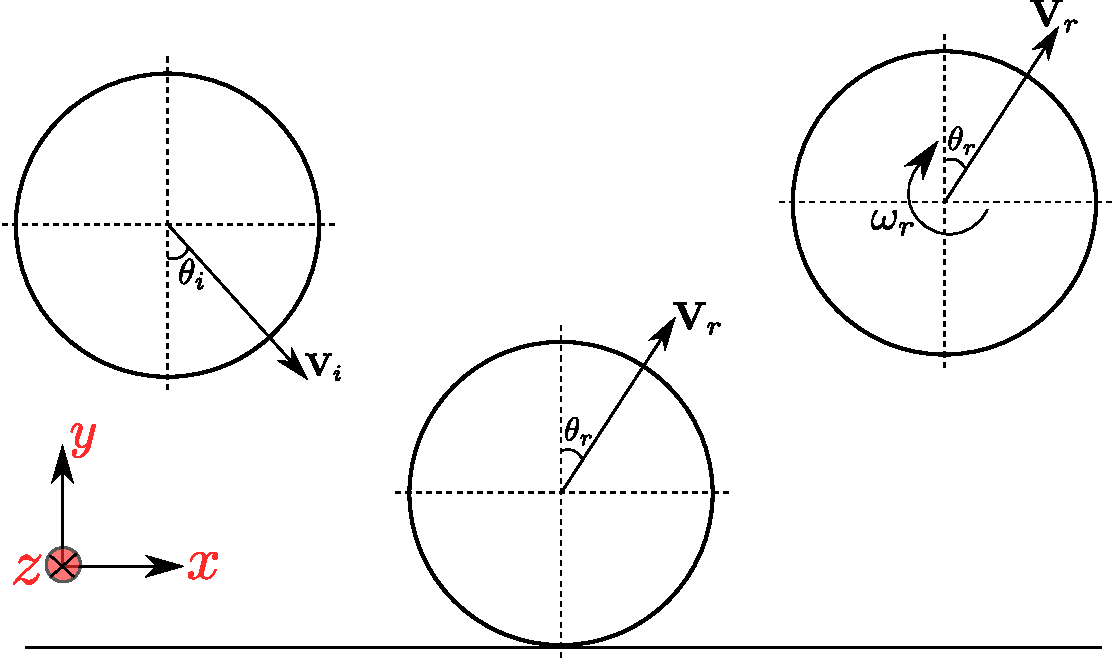
\includegraphics[width=0.6\textwidth]{images/results_dem_2_validation_particle_wall_impact/schematic}
    \subcaption{
    }\label{fig:result:dem-1a}
  \end{subfigure}
  \begin{subfigure}{0.48\textwidth}
    \centering
    \includegraphics[width=0.6\textwidth]{figures/benchmark_4_sw_colliding_oblique/angle_vs_ang_vel.pdf}
    \subcaption{
    }\label{fig:result:dem-1b}
  \end{subfigure}
  \caption{(a) Schematic of particle-wall impact.  (b)
 Variation of Angular velocity with impact angle.}
\label{fig:result-dem-1}
\end{figure}
We consider the collision of a spherical particle with wall with different
incident angles and a constant velocity in magnitude. This test case is useful
in testing the tangential interaction modeling of our DEM solver.  The schematic
of the body and wall is shown in \cref{fig:result:dem-1a}.  The radius of the
impacting particle is $2.5 \times 10^{-3}$ m and is made of aluminium oxide. The
particle has a Young's modulus of $3.8 \times 10^{11}$ N\,m\textsuperscript{-2}, a
Poisson's ratio of $0.23$, and a density of $4,000$
kg\,m\textsuperscript{-3}. The wall's Young's modulus is $70\times 10^{9}$
N\,m\textsuperscript{-2}, with a Poisson's ratio of $0.25$.  The impact velocity
has a magnitude of $3.9$ m\,s\textsuperscript{-1}. The coefficient of friction
between the wall and the particle is $0.092$.  In
\cref{fig:result:dem-1b}, we show variation of the
rebound angular velocity with the incident impact angle, compared to
experimental data.

\FloatBarrier%
\subsection{Single particle entering into a tank}
\label{sec:rfc_validation_1_single_particle_entry}
\begin{figure}[!htpb]
  \centering
  \begin{subfigure}{0.48\textwidth}
    \centering
    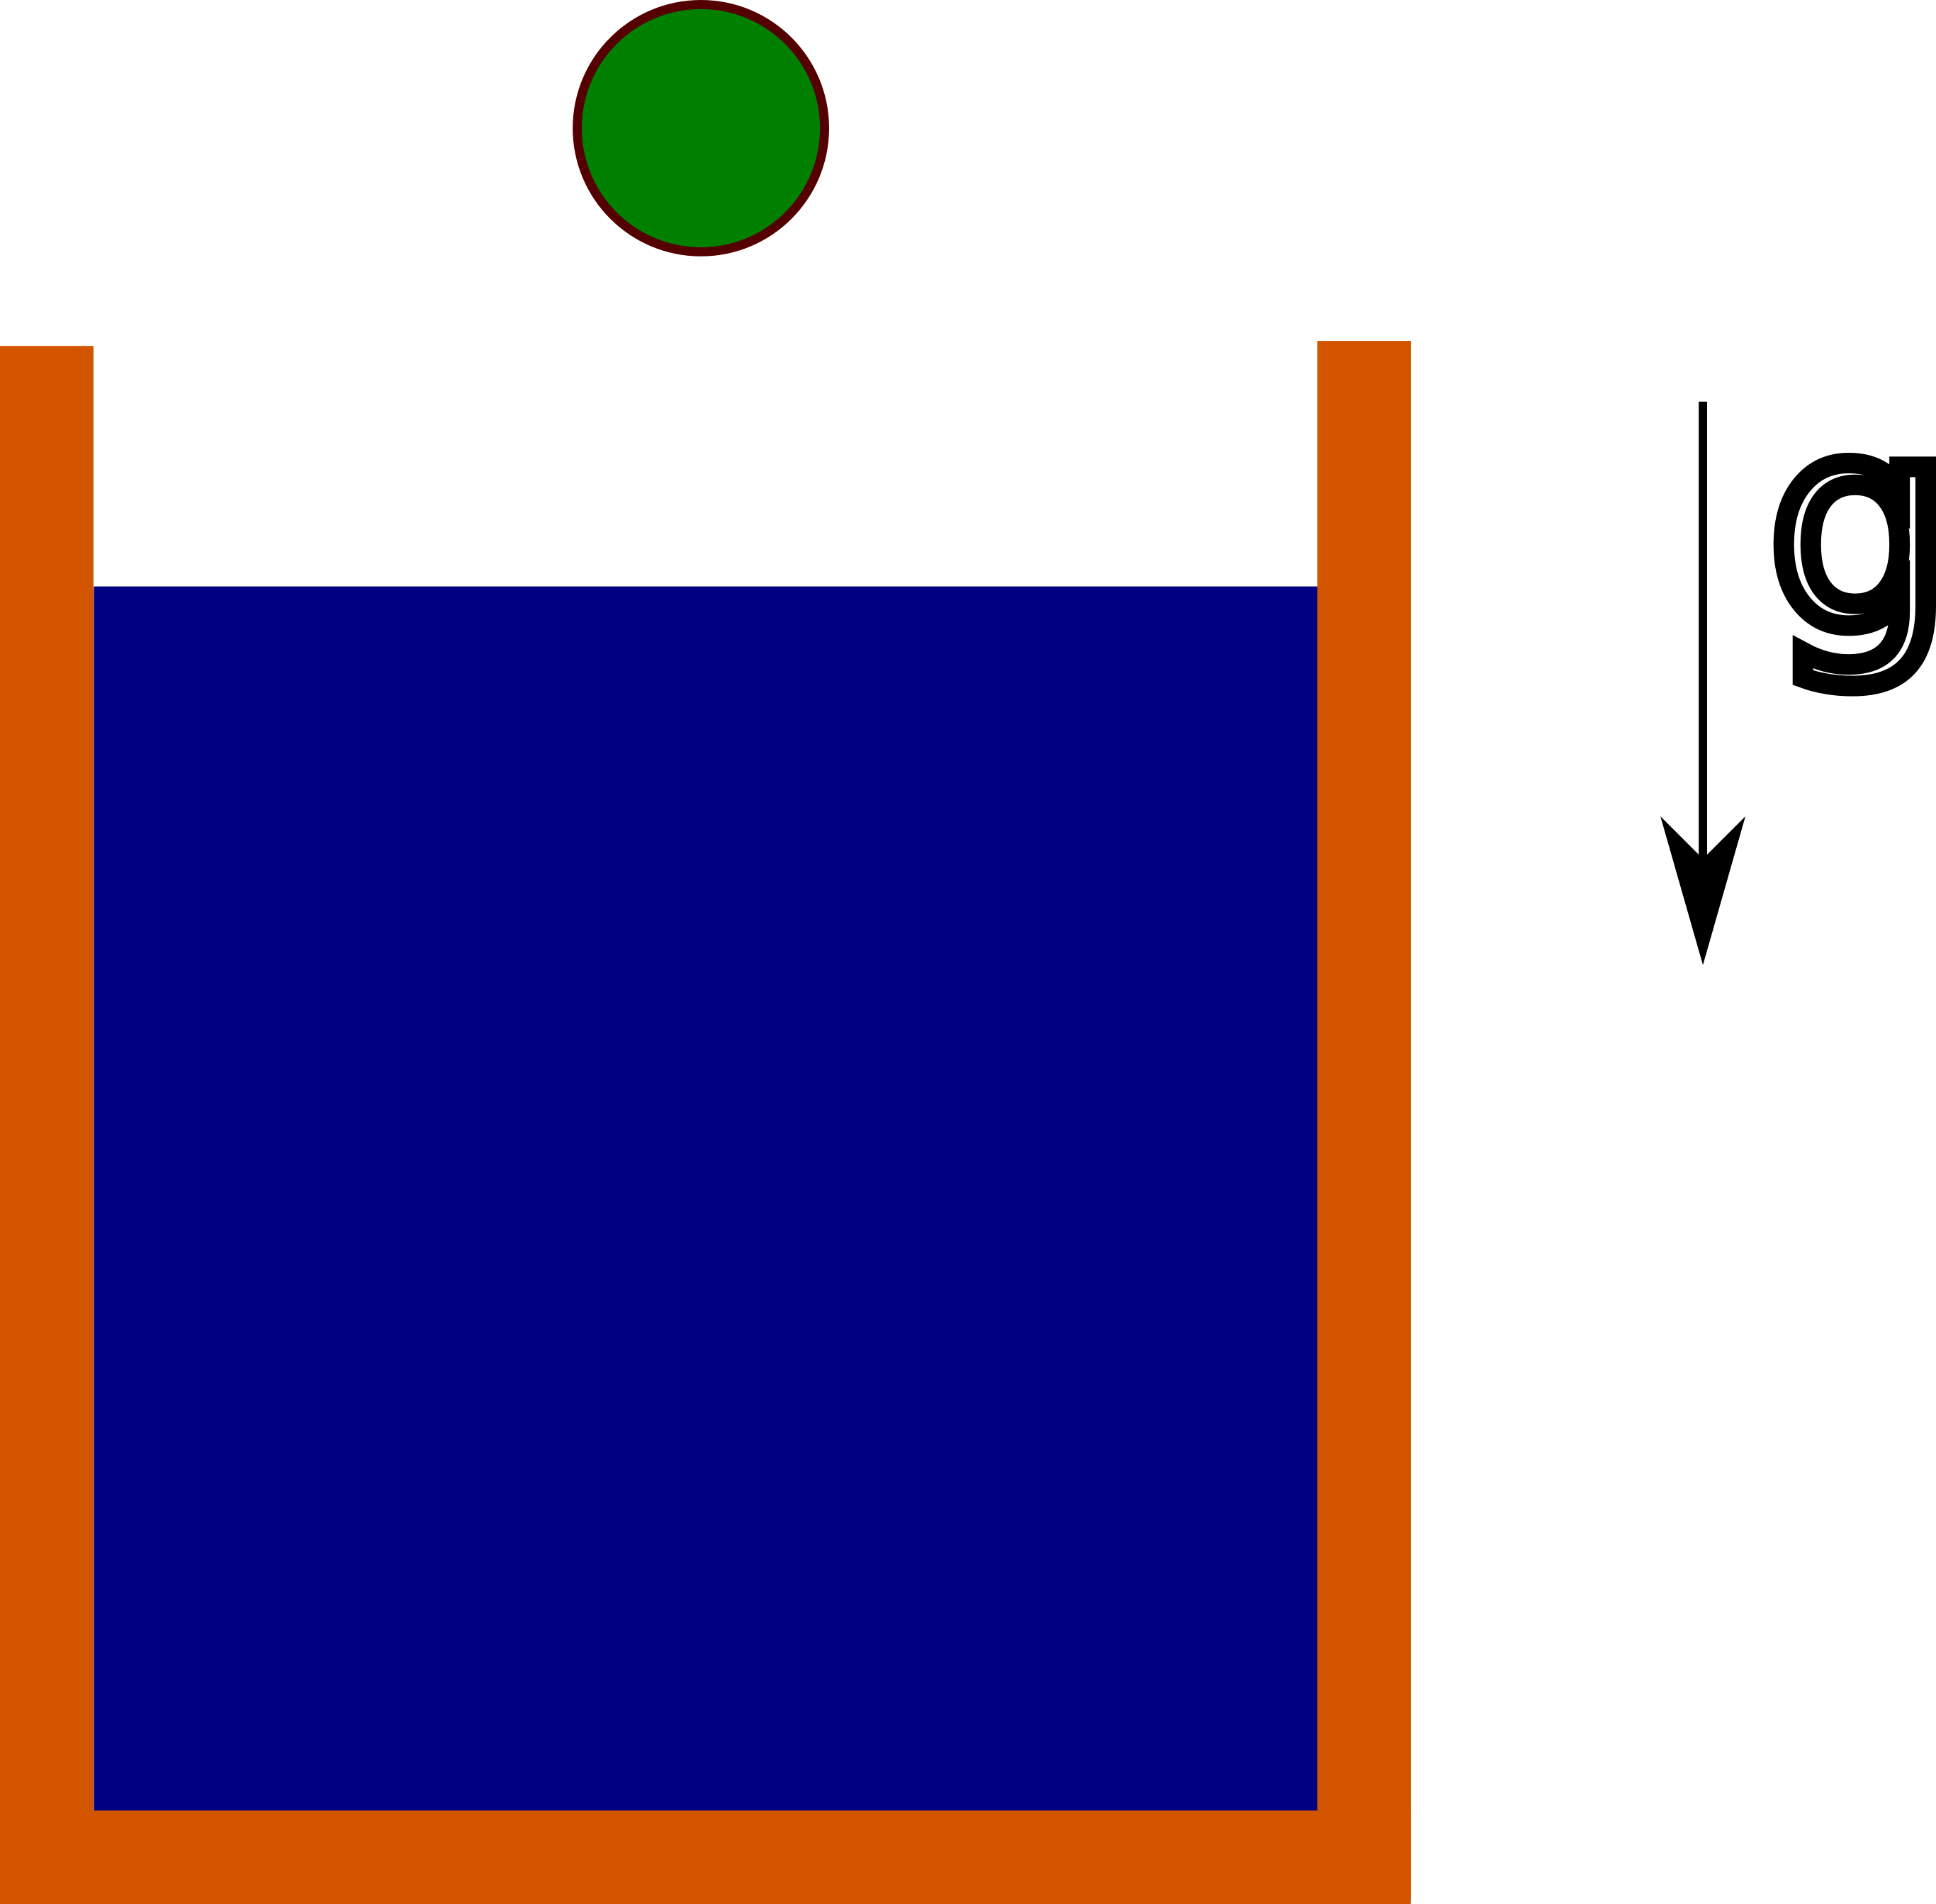
\includegraphics[width=0.6\textwidth]{
      images/rfc_01_skillen_2013_particle_entry_in_hs_tank/Skillen_2013_particle_entry_in_hs_tank}
    \subcaption{}\label{fig:result:rfc-1a}
  \end{subfigure}
  \begin{subfigure}{0.48\textwidth}
    \centering
    \includegraphics[width=0.6\textwidth]{figures/skillen_2013_water_entry_half_buoyant/penetration_vs_t}
    \subcaption{}\label{fig:result:rfc-1b}
  \end{subfigure}
  \caption{(a) Schematic of cylinder disc entering a 2D tank.  (b) Evolution of
    the penetration depth of the cylinder disc with time. }
\label{fig:result-rfc-1}
\end{figure}
In this example we examine the motion of a circular disc descending into a
steady hydrostatic tank. \Cref{fig:result:rfc-1a} illustrates the initial setup,
with the cylinder positioned $0.5$ meters from the free surface. The cylinder's
radius is $0.11$ meters, and density of $500$ kg\,m\textsuperscript{-3}.
\Cref{fig:result:rfc-1b}, depicts the evolution of the depth of penetration of
the cylinder compared to experimental results and other numerical techniques.



% \FloatBarrier%
\subsection{Mixing of spherical particles in a fluid tank}
\label{sec:mixing-spherical-particles-in-fluid-tank-homogeneous}
In this section, we investigate particle dispersion within a tank under various
stirrer velocities. Each circular particle has a radius of $0.055$ m, with a
total of $54$ particles.  The density of the particles is taken as $1050$
kg\,m\textsuperscript{-3}.  After allowing the particles to settle for $1$
second, the stirrer oscillates throughout the fluid length. We examine three
stirrer speeds.  The schematic of the figure is given in
\Cref{fig:1-mixing-1-a}.  \Cref{fig:1-mixing-1-b,fig:1-mixing-1-c,fig:1-mixing-1-d},
illustrate the distribution of particles within a fluid tanker under the
influence of a stirrer at different instants. From \Cref{fig:1-mixing-1},
particles tend to aggregate and settle gradually into a clump at the center.


\section{Conclusions}
This study uses a fully resolved SPH-DEM solver to analyze mixing in a 2D tank
with a stirrer.  SPH simulates the fluid, while DEM handles the
spherical particles and their interactions.  We validated the SPH and DEM
solvers independently and then validated the combined solver with specific test
cases. Finally, we investigated how stirrer speed affects particle dispersion,
finding that both low and high speeds affect the mixing of particles due to the
recirculation and clump formation.

% [!htpb]
\begin{figure}
  \centering
  \begin{subfigure}{0.48\textwidth}
    \centering
    \includegraphics[width=1.0\textwidth]{figures/dinesh_2024_mixing_with_stirrer_homogeneous_2d/case_1/time0}
    \subcaption{t = $0$ s}\label{fig:1-mixing-1-a}
  \end{subfigure}
  \begin{subfigure}{0.48\textwidth}
    \centering
    \includegraphics[width=1.0\textwidth]{figures/dinesh_2024_mixing_with_stirrer_homogeneous_2d/case_1/time1}
    \subcaption{t = $3$ s}\label{fig:1-mixing-1-b}
  \end{subfigure}
  \begin{subfigure}{0.48\textwidth}
    \centering
    \includegraphics[width=1.0\textwidth]{figures/dinesh_2024_mixing_with_stirrer_homogeneous_2d/case_1/time2}
    \subcaption{t = $6$ s}\label{fig:1-mixing-1-c}
  \end{subfigure}
  \begin{subfigure}{0.48\textwidth}
    \centering
    \includegraphics[width=1.0\textwidth]{figures/dinesh_2024_mixing_with_stirrer_homogeneous_2d/case_1/time3}
    \subcaption{t = $9.9$ s}\label{fig:1-mixing-1-d}
  \end{subfigure}
  \caption{Snapshots of fluid, stirrer and the rigid circular particles at
    three time steps, where the stirrer is oscillating at a velocity of $1$
    m\,s\textsuperscript{-1}. The colour contour of the fluid particles
    represents the velocity magnitude.}
\label{fig:1-mixing-1}
\end{figure}
% \begin{figure}[!htpb]
%   \centering
%   \begin{subfigure}{0.48\textwidth}
%     \centering
%     \includegraphics[width=1.0\textwidth]{figures/dinesh_2024_mixing_with_stirrer_homogeneous_2d/case_2/time1}
%     \subcaption{t = $3$ s}\label{fig:1-mixing-1-a}
%   \end{subfigure}
%   \begin{subfigure}{0.48\textwidth}
%     \centering
%     \includegraphics[width=1.0\textwidth]{figures/dinesh_2024_mixing_with_stirrer_homogeneous_2d/case_2/time2}
%     \subcaption{t = $6$ s}\label{fig:1-mixing-1-b}
%   \end{subfigure}

%   \begin{subfigure}{0.48\textwidth}
%     \centering
%     \includegraphics[width=1.0\textwidth]{figures/dinesh_2024_mixing_with_stirrer_homogeneous_2d/case_2/time3}
%     \subcaption{t = $9.9$ s}\label{fig:1-mixing-1-c}
%   \end{subfigure}
%   \caption{Snapshots of fluid, stirrer and the rigid circular particles at
%     three time steps, where the stirrer is oscillating at a velocity of $3$
%     m\,s\textsuperscript{-1}. The colour contour of the fluid particles
%     represents the velocity magnitude.}
% \label{fig:1-mixing-2}
% \end{figure}
% \begin{figure}[!htpb]
%   \centering
%   \begin{subfigure}{0.48\textwidth}
%     \centering
%     \includegraphics[width=1.0\textwidth]{figures/dinesh_2024_mixing_with_stirrer_homogeneous_2d/case_3/time1}
%     \subcaption{t = $3$ s}\label{fig:1-mixing-1-a}
%   \end{subfigure}
%   \begin{subfigure}{0.48\textwidth}
%     \centering
%     \includegraphics[width=1.0\textwidth]{figures/dinesh_2024_mixing_with_stirrer_homogeneous_2d/case_3/time2}
%     \subcaption{t = $6$ s}\label{fig:1-mixing-1-b}
%   \end{subfigure}

%   \begin{subfigure}{0.48\textwidth}
%     \centering
%     \includegraphics[width=1.0\textwidth]{figures/dinesh_2024_mixing_with_stirrer_homogeneous_2d/case_3/time3}
%     \subcaption{t = $9.9$ s}\label{fig:1-mixing-1-c}
%   \end{subfigure}
%   % \begin{subfigure}{0.45\textwidth}
%   %   \centering
%   %   \includegraphics[width=1.0\textwidth]{figures/dinesh_2024_mixing_with_stirrer_homogeneous_2d/case_1/time0}
%   %   \subcaption{t = $7.38$ ms}\label{fig:1-mixing-1-d}
%   % \end{subfigure}
%   \caption{Snapshots of fluid, stirrer and the rigid circular particles at
%     three time steps, where the stirrer is oscillating at a velocity of $5$
%     m\,s\textsuperscript{-1}. The colour contour of the fluid particles
%     represents the velocity magnitude.}
% \label{fig:1-mixing-3}
% \end{figure}


% \section*{Acknowledgments}

% Acknowledgments of your work.
%
% \begin{thebibliography}{99}
% 	\bibitem{Paper}
% 	AutorA, A., AutorB, B., Title of the paper
% 	{\em Name of the Journal}, Volume(Number):Initial Page--Final Page, Year.

% 	\bibitem{Book} BookAuthor, A., Title of the Book. City, Editorial, Year.
% \end{thebibliography}

\bibliographystyle{model6-num-names}
% \bibliography{references}

\end{document}